\documentclass[12pt, a4paper]{article}
\usepackage{xeCJK}
\usepackage{ctex}
\usepackage{cite}
\usepackage{times}
\usepackage{geometry}
\usepackage{fancyhdr}
\usepackage{amsmath}
\usepackage{graphicx}
\usepackage{booktabs}
\usepackage{caption}
\usepackage{setspace}
\usepackage{subcaption}
\usepackage{fancybox}
\usepackage{minipage-marginpar}
\usepackage{amsfonts}
\usepackage{amssymb}
\usepackage{enumitem}
\usepackage{natbib}
\usepackage{titlesec}

\setmainfont{Times New Roman}

\geometry{a4paper, left=1in, right=1in, top=1in, bottom=1in}
\setlength{\parskip}{0pt}
\renewcommand{\baselinestretch}{1.25}

\fancypagestyle{main}{
  \fancyhf{} 
  \fancyhead[L]{\vbox{\hbox to \headwidth{\hfil 多因素视角下的上证380指数收益率动态分析 \hfil}}\line(0,1){\plainlineheight}} 
  \fancyhead[R]{\thepage} 
  \renewcommand{\headrulewidth}{0pt} 
}

\fancypagestyle{main}{
  \fancyhf{}
  \fancyhead[L]{多因素视角下的上证380指数收益率动态分析}
  \fancyhead[R]{\thepage}
}

\newlength{\plainlineheight}
\setlength{\plainlineheight}{0.4pt}

\raggedbottom

\titleformat{\section}{\centering\heiti\zihao{3}}{\thesection}{1em}{}
\titlespacing{\section}{0pt}{0pt}{12pt}  % 确保章节标题在一页的首行居中

\titleformat{\subsection}{\songti\zihao{4}}{\thesubsection}{1em}{}
\titlespacing{\subsection}{0pt}{12pt}{0pt}

\titleformat{\subsubsection}{\heiti\zihao{5}}{\thesubsubsection}{1em}{}
\titlespacing{\subsubsection}{0pt}{12pt}{0pt}

\setCJKmainfont[BoldFont=SimHei]{SimSun}
\newcommand{\song}{\CJKfamily{song}}
\newcommand{\hei}{\CJKfamily{hei}}

\captionsetup[table]{
  font={small,bf},
  labelfont={small,bf},
  labelsep=space,
  textfont={small,bf},
  aboveskip=0pt,
  belowskip=12pt,
}
\captionsetup[figure]{
  font={small,bf},
  labelfont={small,bf},
  labelsep=space,
  textfont={small,bf},
  aboveskip=12pt,
  belowskip=0pt,
}

\renewcommand{\figurename}{图}
\renewcommand{\tablename}{表}

\numberwithin{equation}{section}

\begin{document}

\pagenumbering{roman}
\setcounter{page}{1}
\pagestyle{plain}

\newpage
\begin{center}
    {\heiti \zihao{2} 摘要}
\end{center}
\zihao{-4}

本文采用多元线性回归和GARCH模型,对上证380指数收益率的影响因素及其波动性进行了全面分析。研究表明,上证指数收益率及金融机构新增贷款额对上证380指数收益率具有显著影响。通过对异方差、自相关性和多重共线性进行检测和调整,本研究确保了模型的稳健性。GARCH模型进一步展示了上证指数收益率波动的自相关特性和动态变化模式,为投资者和政策制定者提供了关于市场风险管理的新视角。

\vspace{24pt} % 增加间距

{\heiti \zihao{-4} 关键词:}上证380指数,收益率,影响因素,多元线性回归,GARCH模型,时间序列分析,经济变量

\vspace{36pt} % 增加间距

\begin{center}
    {\bfseries \fontsize{18}{21.6} \selectfont Abstract}
\end{center}
\fontsize{12}{14.4} \selectfont

This paper employs multiple linear regression and GARCH models to conduct a comprehensive analysis of the factors influencing the SSE 380 Index returns and their volatility. The study indicates that the SSE Index returns and the amount of new loans by financial institutions have a significant impact on the returns of the SSE 380 Index. By detecting and adjusting for heteroscedasticity, autocorrelation, and multicollinearity, this research ensures the robustness of the models. Furthermore, the GARCH model elucidates the autocorrelation characteristics and dynamic patterns of volatility in the SSE Index returns, offering new insights into market risk management for investors and policymakers.

\vspace{24pt} % 增加间距

{\bfseries \fontsize{12}{14.4} \selectfont Keywords:} SSE 380 Index, Returns, Influencing Factors, Multiple Linear Regression, GARCH Model, Time Series Analysis, Economic Variables

\renewcommand{\contentsname}{\centering \heiti \zihao{2} 目录}

\newpage
\setlength{\parskip}{0pt}
\tableofcontents

\newpage
\pagestyle{main}
\pagenumbering{arabic}

\section{引言}
\subsection{研究背景与意义}
股市作为国家经济的晴雨表,不仅反映了经济活动的繁荣与衰退,也是投资者情绪和市场预期的直接体现。金融研究领域始终将股市作为研究的重点,试图通过各种分析方法来预测市场走势,为投资决策提供科学依据。特别是在全球化的今天,股市的波动更加复杂多变,研究其内在规律显得尤为重要。

中国股市由于其独特的交易制度和市场环境,例如涨跌停板制度、T+1交易规则等,与西方成熟市场有着明显的区别。这些特点使得中国股市在运行机制、投资者结构和市场效率等方面具有特殊性,从而成为了国内外学者研究的热点。随着中国经济的快速发展和资本市场的逐步开放,中国股市的国际影响力日益增强,对全球金融市场的波动也产生了不可忽视的影响。

上证380指数作为反映上海证券交易所中小型上市公司股票整体表现的重要指标,涵盖了医药、信息技术、消费等多个行业,是投资者观察市场动向和进行资产配置的重要工具。该指数的波动性不仅关系到中小投资者的利益,也对机构投资者的组合管理具有指导意义。然而,由于多种因素的影响,如宏观经济政策、行业发展状况、市场情绪等,上证380指数的收益率波动具有较高的不确定性。因此,研究上证380指数的动态变化对于投资者和市场分析师来说至关重要。深入分析这些波动背后的因素,不仅可以帮助投资者更好地理解市场动态,还可以为政策制定者提供制定有效市场监管政策的依据。

\subsection{论文结构}
本研究从多因素视角出发,运用多元线性回归、GARCH模型、时间序列分析等定量研究方法,对上证380指数的收益率波动进行了全面而深入的分析。研究首先通过文献综述,系统梳理了国内外学者在股市收益率影响因素方面的研究成果,为本研究提供了理论基础和方法论指导。随后,研究基于锐思数据库和国家统计局的数据,对上证380指数及其相关经济变量进行了描述性统计和时间序列图的绘制,为实证分析打下了数据基础。

在实证分析阶段,研究构建了多元线性回归模型,将上证指数收益率、沪市A股市场月总市值、人民币对美元汇率、金融机构新增贷款金额、居民消费价格指数和货币供应量等作为解释变量,以上证380指数收益率为被解释变量,探讨了这些因素对指数收益率的影响。通过模型估计和统计检验,研究揭示了各因素对上证380指数收益率的作用机制和影响力度。

此外,研究还对模型的异方差性、自相关性、多重共线性等问题进行了检验和修正,确保了分析结果的稳健性。GARCH模型的引入,进一步分析了上证指数收益率的波动性特征,为理解市场风险提供了新的视角。

最终,研究结果表明,上证指数收益率和金融机构新增贷款金额对上证380指数收益率有显著影响,其中上证指数收益率对上证380指数收益率具有正向作用,而金融机构新增贷款金额则呈现负向影响。同时,研究还指出了模型和数据方面的局限性,并对未来研究方向提出了建议,如引入非线性模型、使用更高频率的数据、扩展到其他股票市场以及结合重大经济事件进行研究等,以期获得更加全面和深入的理解。

\newpage
\section{文献综述与模型理论基础}
\subsection{国内外关于股票指数收益率影响因素的研究}
股票指数收益率作为金融市场研究的关键议题,吸引了众多学者的广泛关注。他们从多元化的视角出发,深入探讨了影响股票指数收益率的多种因素。例如,于雪皎在其研究中深入分析了上证指数的收益率波动特性,揭示了股票价格收益率的“尖峰厚尾”统计特征及其异方差性[1]。顾鹏则利用中国A股市场的日度数据,探究了宏观经济冲击对股票收益率的作用,发现工业增加值和生产者物价指数对上海及深圳主板市场股票收益率具有显著的影响[2]。杨科等人采用向量自回归模型,研究了中国股票市场收益率与波动率之间的因果联系,揭示了明显的动态杠杆效应[3]。

此外,李腊生等学者则从理论层面剖析了收益率分布时变性的微观经济基础,并结合中国上证指数的实际数据,验证了股票收益率分布时变性的现实存在[4]。王元月和梁翠翠运用状态空间模型,对流动性与上证综指收益率之间的动态关系进行了细致的变参数分析,指出上证综指收益率对宏观流动性变动的时变弹性系数近年来呈现上升趋势[5]。而陈守东等通过Granger因果检验和GARCH-M模型,深入分析了沪深股市收益率及波动性的相关性,结果表明两市收益率之间具有强烈的相关性,并且均存在显著的风险溢价[6]。

在对上证综指波动特征及其收益率影响因素的研究中,王晓芳和王瑞君基于经验模态分解(EEMD)和向量自回归(VAR)模型的分析,发现M2货币供应量的增长率是影响上证综指低频分量和趋势项收益率的长期主导因素[7]。

综合国内外研究,股票指数收益率受多种因素影响,包括宏观经济指标、市场内部波动性以及流动性状况。这些研究不仅揭示了市场波动的统计特性和动态因果关系,还强调了宏观经济与市场流动性对股票收益的显著影响。特别是,货币供应量增长率与长期股票收益率趋势的关联,为投资者和政策制定者提供了重要的视角。
\subsection{相关理论基础与模型介绍}
本小节分析上证380指数收益率的主要理论模型,包括多元线性回归模型和GARCH模型。

多元线性回归模型是金融计量经济学中常用的统计模型,用于描述一个因变量与多个自变量之间的线性关系。其模型表达式如公式2-1所示。
\begin{equation}
    Y = \beta_0 + \beta_1X_1 + \beta_2X_2 + \cdots + \beta_nX_n + \epsilon \tag{2-1}
\end{equation}
其中,$Y$ 表示被解释变量,$X_1, X_2, \ldots, X_n$ 表示解释变量,$\beta_0, \beta_1, \ldots, \beta_n$ 为模型参数,$\epsilon$ 为误差项。

GARCH模型被广泛应用于金融时间序列数据的波动性分析。该模型能够有效捕捉金融数据的波动聚集现象。基本形式如公式2-2所示。
\begin{equation}
    \left\{
    \begin{aligned}
         & \text{均值方程:}   & Y_t        & = \beta_1X_t + \epsilon_t,                                \\
         & \text{条件方差方程:} & \sigma_t^2 & = \omega + \alpha \epsilon_{t-1}^2 + \beta \sigma_{t-1}^2
    \end{aligned}
    \right. \tag{2-2}
\end{equation}

其中,$\sigma_t^2$ 表示时间$t$的条件方差,$\epsilon_{t-1}$是前一期的残差,$\omega, \alpha, \beta$ 是模型参数。

这两个模型在实证分析中具有重要应用,其中多元线性回归模型可以帮助我们估计不同因素对上证380指数收益率的影响程度,而GARCH模型则用于研究收益率的波动特征。

\newpage
\section{数据来源与描述性统计}

\subsection{数据来源说明}
本文使用的数据来源于锐思数据库和国家统计局。锐思数据库提供了上证380指数(000009)的月度收益率数据,以及上证指数(000001)月度收益率、沪市A股市场月总市值、人民币对美元汇率和金融机构新增贷款金额等指标的数据。居民消费价格指数和货币和准货币供应量期末值则来源于国家统计局。表3.1是各个变量的简称和含义表。

\begin{table}[h!]
    \centering
    \captionsetup{labelformat=empty}
    \caption{\textbf{\fontsize{9pt}{11pt}\selectfont 表3.1 变量简称和含义表}}
    \begin{tabular}{lcl}
        \toprule
        数据名称       & 简称       & 含义                     \\
        \midrule
        上证380指数收益率 & R\_SZ380 & 上证380指数的月度收益率          \\
        上证指数收益率    & R\_SZ    & 上证指数(000001)的月度收益率     \\
        沪市A股市场月总市值 & MC\_SH   & 沪市A股市场的月总市值            \\
        人民币对美元汇率   & INTEREST & 期平均;直接标价法,单位:人民币元/1美元  \\
        金融机构新增贷款金额 & LOAN     & 金融机构新增贷款金额(数据以截止日期为基准) \\
        居民消费价格指数   & CPI      & 居民消费价格指数               \\
        货币和准货币供应量  & M2       & 货币和准货币供应量期末值           \\
        \bottomrule
    \end{tabular}
\end{table}


\subsection{描述性统计表的构建与分析}
首先,为了对数据有一个初步的了解,我们对所有变量进行了描述性统计分析。描述性统计表包括变量的均值、中位数、最大值、最小值和标准差等指标。以下是描述性统计结果表。

\begin{table}[h!]
    \centering
    \captionsetup{labelformat=empty}
    \caption{\textbf{\fontsize{9pt}{11pt}\selectfont 表3.2 变量描述性统计表}}
    \begin{tabular}{lccccc}
        \toprule
        变量       & 均值        & 中位数       & 最大值      & 最小值       & 标准差      \\
        \midrule
        CPI      & 100.1436  & 100.1000  & 101.6000 & 98.8000   & 0.507060 \\
        INTEREST & 6.744132  & 6.754800  & 7.183900 & 6.297500  & 0.249008 \\
        LOAN     & 15617.72  & 12550.00  & 69700.00 & 3459.00   & 10250.88 \\
        M2       & 2060776   & 1973959   & 2896659  & 1416320   & 431119.9 \\
        R\_SZ    & -0.000507 & -0.001450 & 0.137900 & -0.226500 & 0.048116 \\
        MC\_SH   & 354662.5  & 334155.8  & 459819.4 & 233593.4  & 64828.21 \\
        R\_SZ380 & -0.000816 & -0.001200 & 0.183600 & -0.282300 & 0.058137 \\
        \bottomrule
    \end{tabular}
\end{table}

表3.2显示了各个变量的基本统计特征。首先,CPI的均值和中位数非常接近,表明数据分布较为对称。标准差较小,说明CPI在不同时间点的波动不大,基本维持在100左右。其次,汇率的均值和中位数也较为接近,数据分布相对对称。标准差略高于CPI,表明汇率在不同时间点有一定的波动,但总体稳定在6.74左右。而新增贷款金额的均值远高于中位数,且最大值和最小值差异较大,表明新增贷款金额数据可能存在一定的偏态分布。标准差较大,显示贷款金额的波动性较大。此外,M2的均值和中位数差异不大,但最大值和最小值差距较大,说明货币供应量在不同时间点的变化幅度较大。标准差也较大,表明货币供应量波动性较高。上证指数收益率的均值接近于0,表明在研究期间内总体收益率几乎没有增长。中位数为负值,说明多数月份的收益率为负。标准差较小,表明上证指数收益率的波动性较小。另外,沪市A股市场总市值的均值和中位数较为接近,表明数据分布较为对称。最大值和最小值差距较大,显示市值在不同时间点的波动性较大。最后,上证380指数收益率的均值为负值,表明在研究期间内总体收益率为负。标准差较小,表明上证380指数收益率的波动性也较小。

\subsection{影响因素的时间序列图绘制与趋势分析}
为了更直观地展示各变量随时间的变化趋势,我们选取了三个变量,并绘制了它们的时间序列图。图3-1至3-3是CPI、M2和R\_SZ的时间序列图。通过时间序列图,可以观察到这些变量随时间的波动情况和趋势变化。这为我们后续的实证分析提供了参考依据。

\begin{figure}[h!]
    \centering
    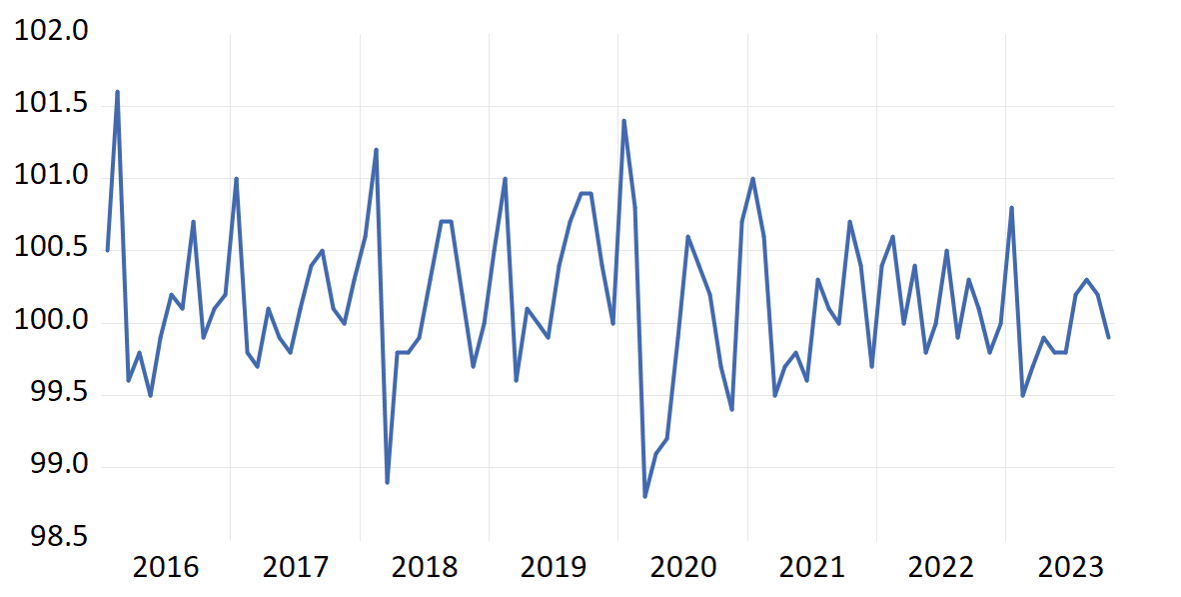
\includegraphics[width=0.75\textwidth]{./img/cpi.png}
    \captionsetup{labelformat=empty}
    \caption{\textbf{\fontsize{9pt}{11pt}\selectfont 图3-1 CPI时间序列图}}
\end{figure}

\begin{figure}[h!]
    \centering
    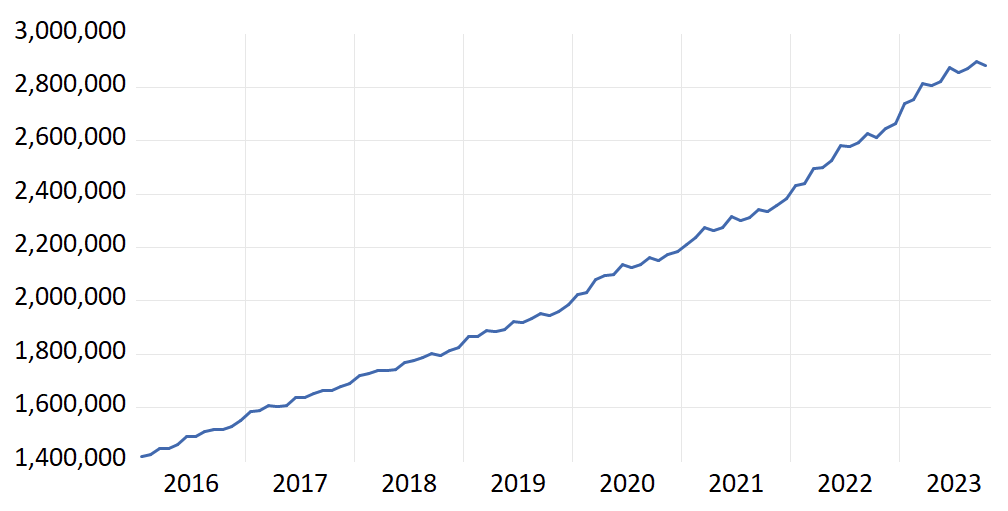
\includegraphics[width=0.75\textwidth]{./img/m2.png}
    \captionsetup{labelformat=empty}
    \caption{\textbf{\fontsize{9pt}{11pt}\selectfont 图3-2 M2时间序列图}}
\end{figure}

\begin{figure}[h!]
    \centering
    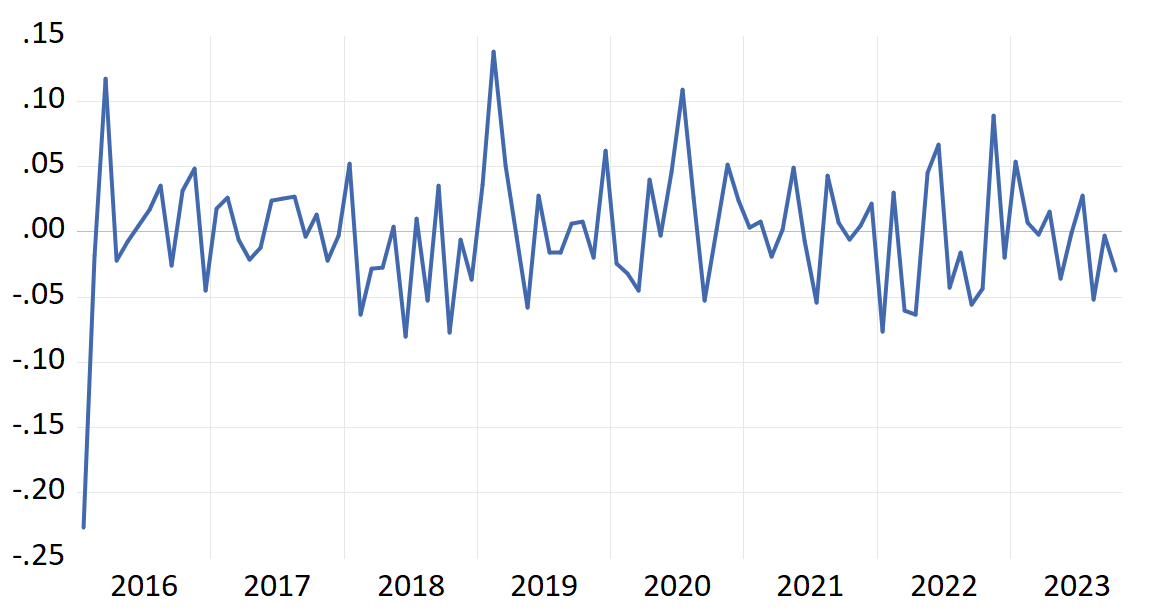
\includegraphics[width=0.75\textwidth]{./img/r_sz.png}
    \captionsetup{labelformat=empty}
    \caption{\textbf{\fontsize{9pt}{11pt}\selectfont 图3-3 R\_SZ时间序列图}}
\end{figure}

\clearpage

\newpage
\section{研究方法与模型构建}
\subsection{多元线性回归模型的构建}
本文利用Eviews软件,构建了一个多元线性回归模型,以上证380指数收益率(R\_SZ380)为被解释变量,选取上证指数(R\_SZ)、沪市A股市场月总市值(MC\_SH)、人民币对美元汇率(INTEREST)、金融机构新增贷款金额(LOAN)、居民消费价格指数(CPI)及货币和准货币供应量(M2)作为解释变量。模型的形式如公式4-1所示。
\begin{equation}
    \begin{aligned}[t]
        R\_SZ380 & = \beta_0 + \beta_1 R\_SZ + \beta_2 MC\_SH                                    \\
                 & \quad + \beta_3 INTEREST + \beta_4 LOAN + \beta_5 CPI + \beta_6 M2 + \epsilon
    \end{aligned}
    \tag{4-1}
\end{equation}

\subsection{模型的假设条件与检验方法}
在构建多元线性回归模型时,本文遵循了以下经典的计量回归假设条件:
\begin{enumerate}[label=\arabic*)]
    \item 线性关系:因变量与自变量之间存在线性关系。
    \item 自变量之间无完全共线性:各自变量之间应无完全的线性关系。
    \item 同方差性:误差项的方差应为常数。
    \item 独立性:误差项之间应相互独立。
    \item 正态性:误差项应服从正态分布。
\end{enumerate}

各项假设条件的检验方法如下:
\begin{enumerate}[label=\arabic*)]
    \item 异方差检验:采用图示法和解析法检验模型是否存在异方差问题,若存在,则进行异方差修正。
    \item 自相关检验:采用图示法和解析法检验模型是否存在自相关问题,若存在,则进行自相关修正。
    \item 多重共线性检验:计算各个解释变量之间的相关系数,并得出相关系数矩阵的行列式,以判断是否存在多重共线性。
    \item 平稳性检验:对所有变量进行平稳性检验,并检验被解释变量与部分解释变量之间是否存在协整关系。
\end{enumerate}

基于上述理论模型、假设条件和检验方法,本文将在下一章进行实证分析。

\newpage
\section{实证分析}
\subsection{多元线性回归分析}
\subsubsection{模型估计结果}
为了分析上证380指数收益率的影响因素,我们采用了多元线性回归模型进行估计。模型的被解释变量是上证380指数收益率(R\_SZ380),解释变量包括居民消费价格指数(CPI)、人民币对美元汇率(INTEREST)、金融机构新增贷款金额(LOAN)、货币和准货币供应量(M2)、沪市A股市场月总市值(MC\_SH)和上证指数收益率(R\_SZ)。

模型的估计结果如表5.1所示。

\begin{table}[h!]
    \centering
    \captionsetup{labelformat=empty}
    \caption{\textbf{\fontsize{9pt}{11pt}\selectfont 表5.1 多元线性回归估计结果}}
    \begin{tabular}{lccccc}
        \toprule
        变量       & 系数        & 标准误      & t值        & Prob.  \\
        \midrule
        常数项 (C)  & 0.156870  & 0.473199 & 0.331509  & 0.7411 \\
        CPI      & -0.000915 & 0.004678 & -0.195600 & 0.8454 \\
        INTEREST & -0.010010 & 0.013456 & -0.743865 & 0.4590 \\
        LOAN     & -4.81E-07 & 2.39E-07 & -2.010308 & 0.0475 \\
        M2       & 1.42E-08  & 1.68E-08 & 0.846313  & 0.3997 \\
        MC\_SH   & -5.59E-08 & 1.07E-07 & -0.521300 & 0.6035 \\
        R\_SZ    & 1.103144  & 0.050006 & 22.06045  & 0.0000 \\
        \bottomrule
    \end{tabular}
\end{table}

根据回归结果,拟合的回归方程如公式5-1所示。

\[
    \begin{aligned}
        R\_{\textit{SZ}380} & = 0.156870 - 0.000915 \times \textit{CPI} \,                                                   \\
                            & \quad - 0.010010 \times \textit{INTEREST} - 4.81 \times 10^{-7} \times \textit{LOAN} \,        \\
                            & \quad + 1.42 \times 10^{-8} \times \textit{M2} - 5.59 \times 10^{-8} \times \textit{MC\_SH} \, \\
                            & \quad + 1.103144 \times \textit{R\_SZ}
    \end{aligned}
    \tag{5-1}
\]

从表5.1可以看出,上证指数收益率(R\_SZ)和金融机构新增贷款金额(LOAN)对上证380指数收益率(R\_SZ380)有显著影响,而其他变量(CPI、INTEREST、M2、MC\_SH)在5\%的显著性水平下不显著。

\subsubsection{模型的统计检验}
为了评估回归模型的整体拟合效果和模型的可靠性,我们还进行了统计检验:首先,模型的R平方值为0.858724,表明模型能够解释约85.87\%的上证380指数收益率的变异性。调整后R平方值为0.848980,进一步验证了模型的拟合效果。其次,模型的F统计量为88.13571,对应的p值为0.000000,表明回归模型整体上是显著的。回归的标准误为0.022593,表示预测误差的平均水平。综上,由统计检验可以看出,模型整体具有较强的解释力,但是还留有一些异方差、自相关等问题,这些问题由后面小节讨论。


\subsection{异方差性检验与修正}
\subsubsection{图示法与解析法判断异方差现象}
为了判断模型是否存在异方差问题,我们首先采用图示法对残差的平方进行散点图分析,如图片组5-1至5-6所示。

\begin{figure}[h!]
    \centering
    \begin{subfigure}{0.45\textwidth}
        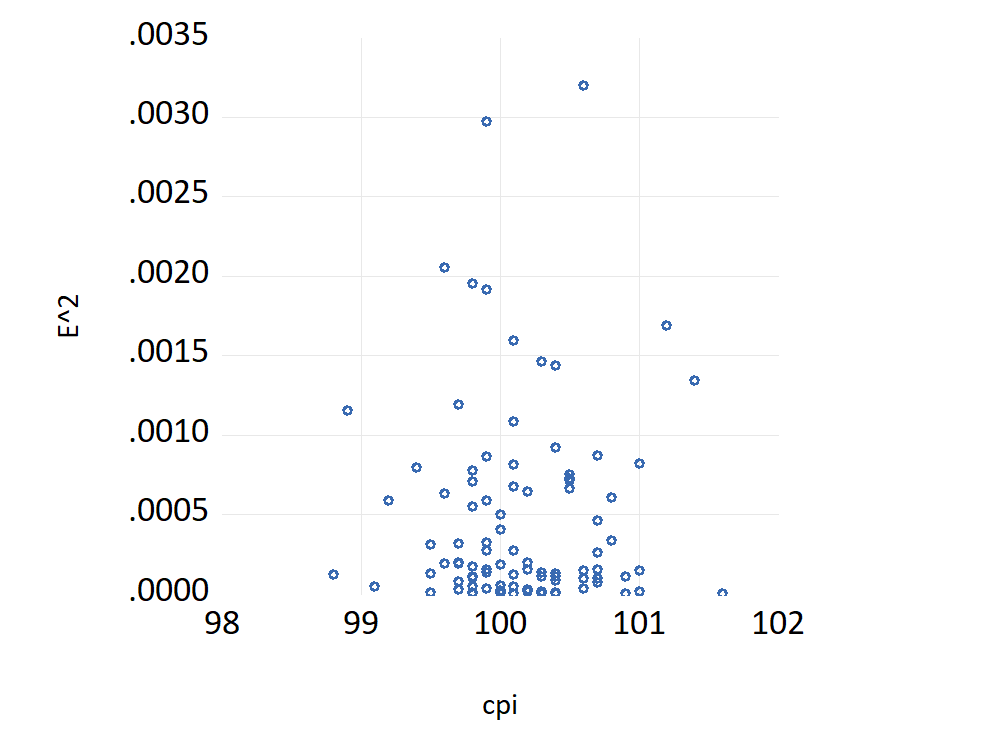
\includegraphics[width=\textwidth]{./img/cpi-e2.png}
        \captionsetup{labelformat=empty}
        \caption{\textbf{\fontsize{9pt}{11pt}\selectfont 图5-1 残差平方与CPI的散点图}}
    \end{subfigure}
    \hspace{0.05\textwidth}
    \begin{subfigure}{0.45\textwidth}
        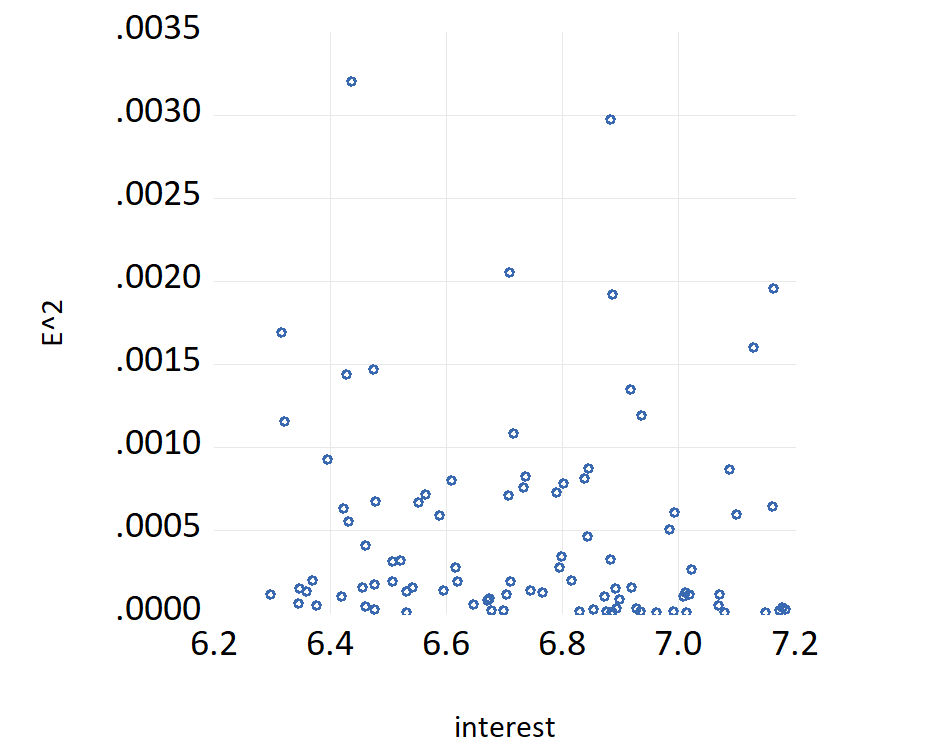
\includegraphics[width=\textwidth]{./img/interest-e2.png}
        \captionsetup{labelformat=empty}
        \caption{\textbf{\fontsize{9pt}{11pt}\selectfont 图5-2 残差平方与INTEREST的散点图}}
    \end{subfigure}
    \vspace{0.05\textwidth}
    \begin{subfigure}{0.45\textwidth}
        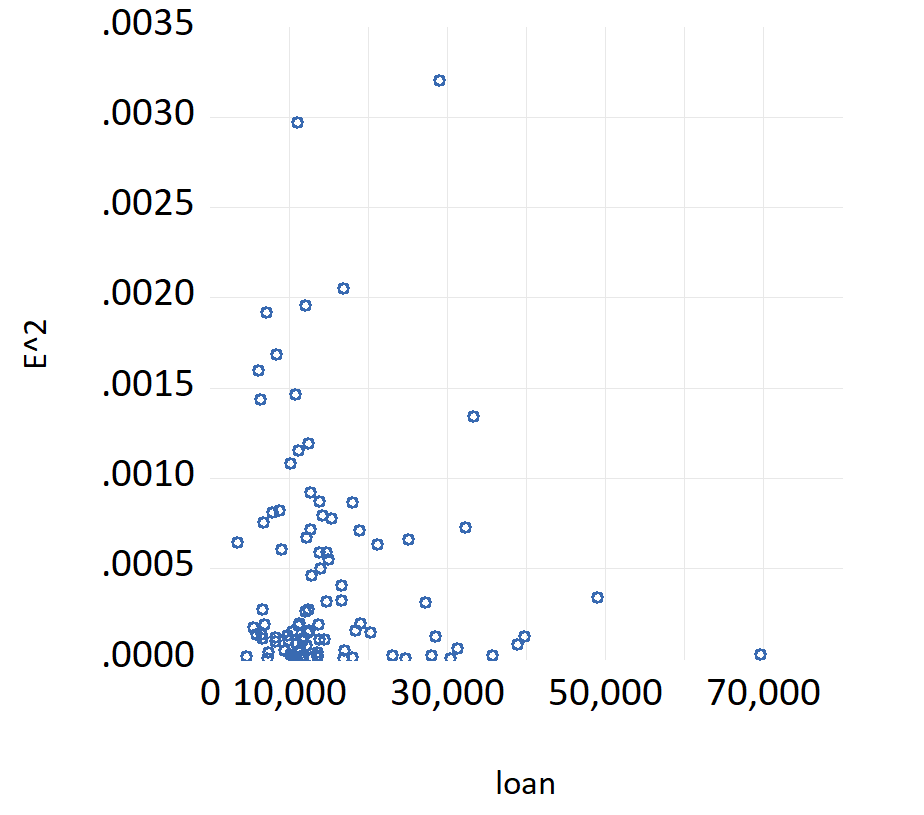
\includegraphics[width=\textwidth]{./img/loan-e2.png}
        \captionsetup{labelformat=empty}
        \caption{\textbf{\fontsize{9pt}{11pt}\selectfont 图5-3 残差平方与LOAN的散点图}}
    \end{subfigure}
    \hspace{0.05\textwidth}
    \begin{subfigure}{0.45\textwidth}
        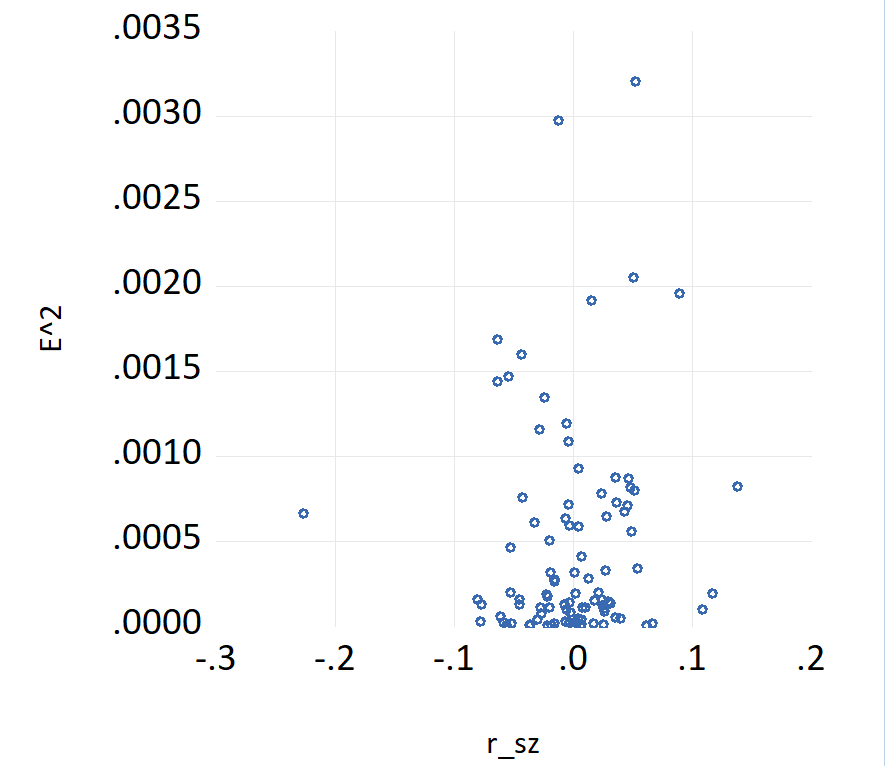
\includegraphics[width=\textwidth]{./img/r_sz-e2.png}
        \captionsetup{labelformat=empty}
        \caption{\textbf{\fontsize{9pt}{11pt}\selectfont 图5-4 残差平方与R\_SZ的散点图}}
    \end{subfigure}
    \vspace{0.05\textwidth}
    \begin{subfigure}{0.45\textwidth}
        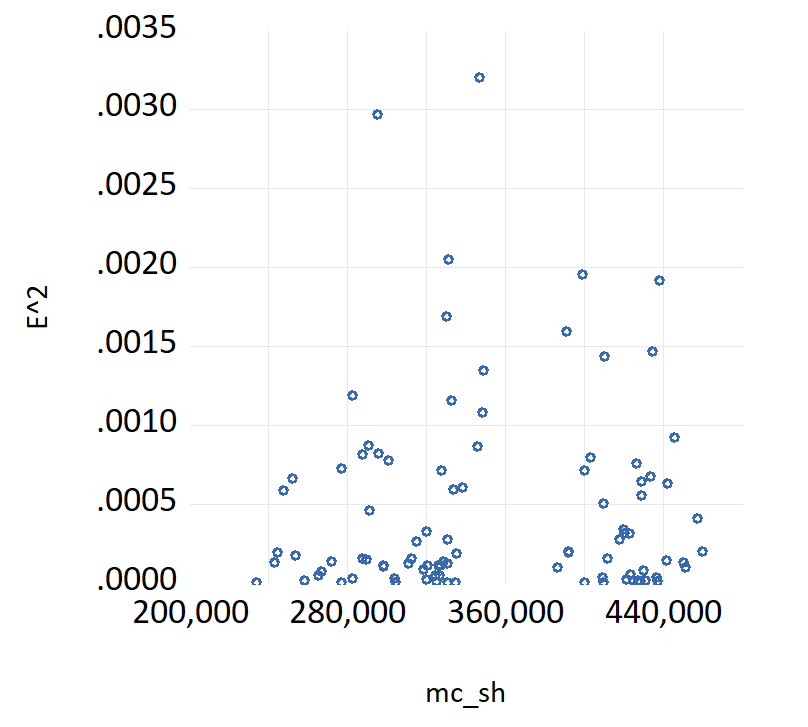
\includegraphics[width=\textwidth]{./img/mc_sh-e2.png}
        \captionsetup{labelformat=empty}
        \caption{\textbf{\fontsize{9pt}{11pt}\selectfont 图5-5 残差平方与MC\_SH的散点图}}
    \end{subfigure}
    \hspace{0.05\textwidth}
    \begin{subfigure}{0.45\textwidth}
        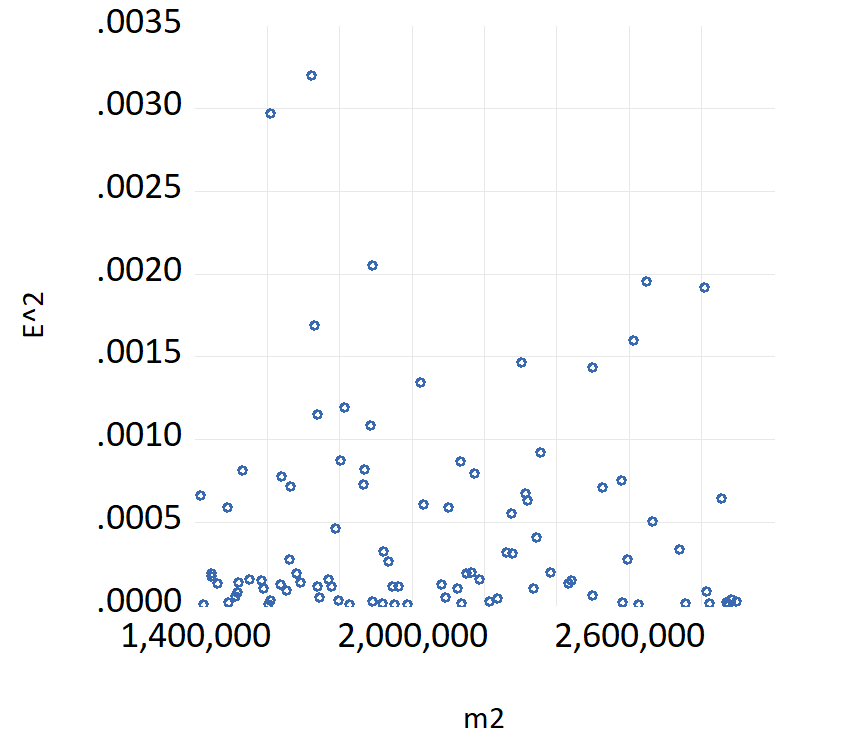
\includegraphics[width=\textwidth]{./img/m2-e2.png}
        \captionsetup{labelformat=empty}
        \caption{\textbf{\fontsize{9pt}{11pt}\selectfont 图5-6 残差平方与M2的散点图}}
    \end{subfigure}
    \captionsetup{labelformat=empty}
\end{figure}

从图中可以看出,残差平方与各个变量之间没有明显的规律性分布,初步判断模型中不存在严重的异方差现象。

接着,我们采用White检验对模型进行异方差性解析法检验。White检验的结果如表5.2所示。

\begin{table}[h!]
    \centering
    \captionsetup{labelformat=empty}
    \caption{\textbf{\fontsize{9pt}{11pt}\selectfont 表5.2 White检验结果}}
    \begin{tabular}{lcccc}
        \toprule
        检验统计量               & 统计量大小    & 自由度      & Prob.  \\
        \midrule
        F统计量                & 1.368976 & (26, 67) & 0.1528 \\
        Obs*R平方             & 32.61202 & 26       & 0.1737 \\
        Scaled explained SS & 24.72145 & 26       & 0.5348 \\
        \bottomrule
    \end{tabular}
\end{table}

根据表5.2,White检验的p值均大于10\%,我们无法拒绝原假设,即认为模型中不存在异方差现象。

\subsubsection{异方差的修正方法}
虽然从图示法和White检验结果来看,模型中并不存在显著的异方差问题,但是p值只是略大于10\%,故为了稳妥起见,我们对模型中的非平稳变量进行了对数变换,并对其进行一阶差分处理,以消除可能的异方差问题。处理后的回归结果如表5.3所示。

\begin{table}[h!]
    \centering
    \captionsetup{labelformat=empty}
    \caption{\textbf{\fontsize{9pt}{11pt}\selectfont 表5.3 对数变换后多元线性回归结果}}
    \begin{tabular}{lccccc}
        \toprule
        变量             & 系数        & 标准误      & t值        & Prob.  \\
        \midrule
        常数项 (C)        & -0.014749 & 0.478854 & -0.030800 & 0.9755 \\
        CPI            & 0.000204  & 0.004780 & 0.042595  & 0.9661 \\
        DLOG\_INTEREST & 0.228841  & 0.217932 & 1.050058  & 0.2966 \\
        DLOG\_M2       & 0.207365  & 0.358148 & 0.578993  & 0.5641 \\
        DLOG\_MC\_SH   & 0.058290  & 0.094594 & 0.616219  & 0.5394 \\
        LOAN           & -4.86E-07 & 2.81E-07 & -1.732202 & 0.0868 \\
        R\_SZ          & 1.040298  & 0.074406 & 13.98147  & 0.0000 \\
        \bottomrule
    \end{tabular}
\end{table}

通过对数变换后的回归结果显示,上证指数收益率(R\_SZ)仍然对上证380指数收益率(R\_SZ380)具有显著影响。

为了验证异方差问题是否得到解决,我们再次采用White检验对处理后的模型进行检验,结果如表5.4所示。

\begin{table}[h!]
    \centering
    \captionsetup{labelformat=empty}
    \caption{\textbf{\fontsize{9pt}{11pt}\selectfont 表5.4 处理后White检验结果}}
    \begin{tabular}{lccc}
        \toprule
        检验统计量               & 统计量大小    & 自由度      & Prob.  \\
        \midrule
        F统计量                & 0.796911 & (26, 66) & 0.7356 \\
        Obs*R平方             & 22.22022 & 26       & 0.6766 \\
        Scaled explained SS & 16.83220 & 26       & 0.9141 \\
        \bottomrule
    \end{tabular}
\end{table}

根据表5.4,处理后的White检验结果显示p值显著增大,进一步验证了通过对数变换和一阶差分处理,模型中的异方差问题得到了有效的解决。


\subsection{自相关性检验与修正}
\subsubsection{自相关性问题的识别}
为了识别模型中是否存在自相关性问题,我们采用图示法和解析法进行检验。

首先,我们通过绘制残差序列图和残差自相关散点图来进行初步判断,如图5-7和图5-8所示。

\begin{figure}[h!]
    \centering
    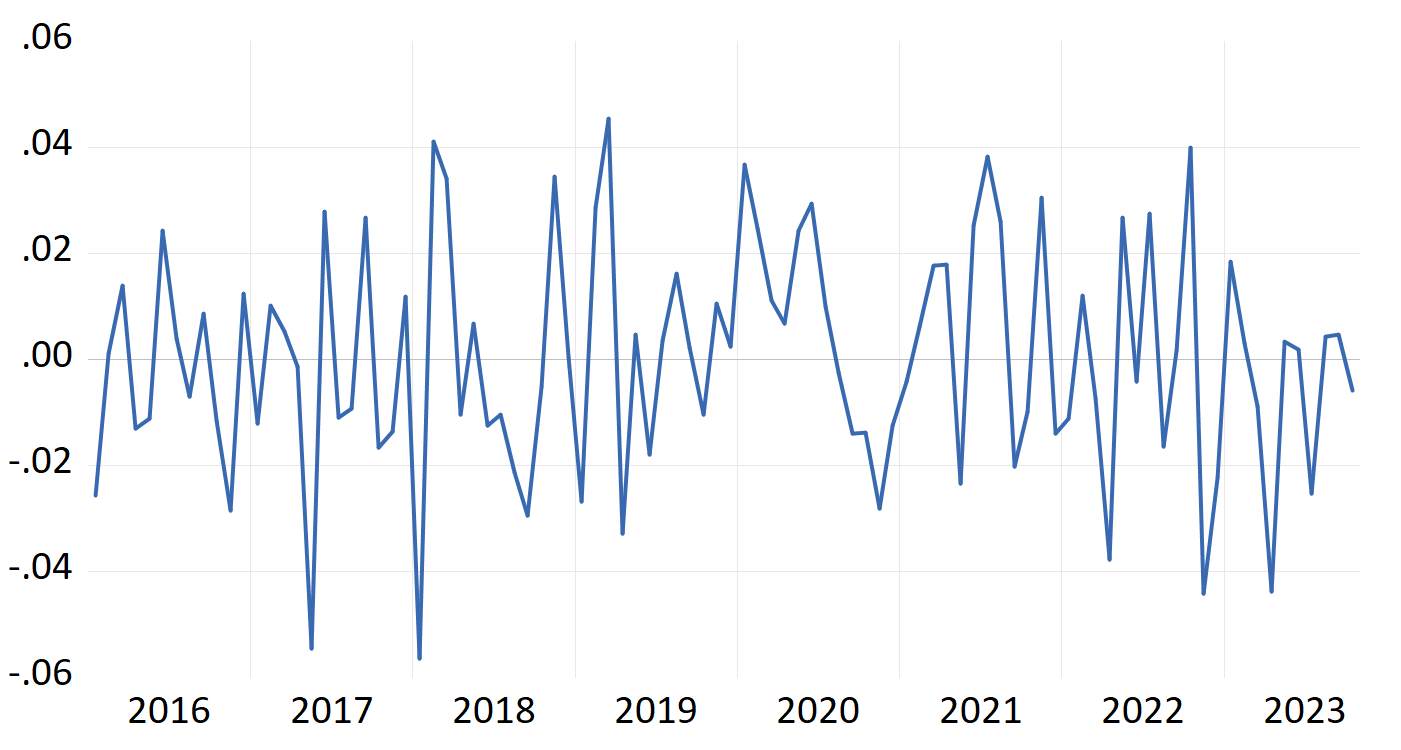
\includegraphics[width=0.75\textwidth]{./img/e.png}
    \captionsetup{labelformat=empty}
    \caption{\textbf{\fontsize{9pt}{11pt}\selectfont 图5-7 残差序列图}}
\end{figure}

\begin{figure}[h!]
    \centering
    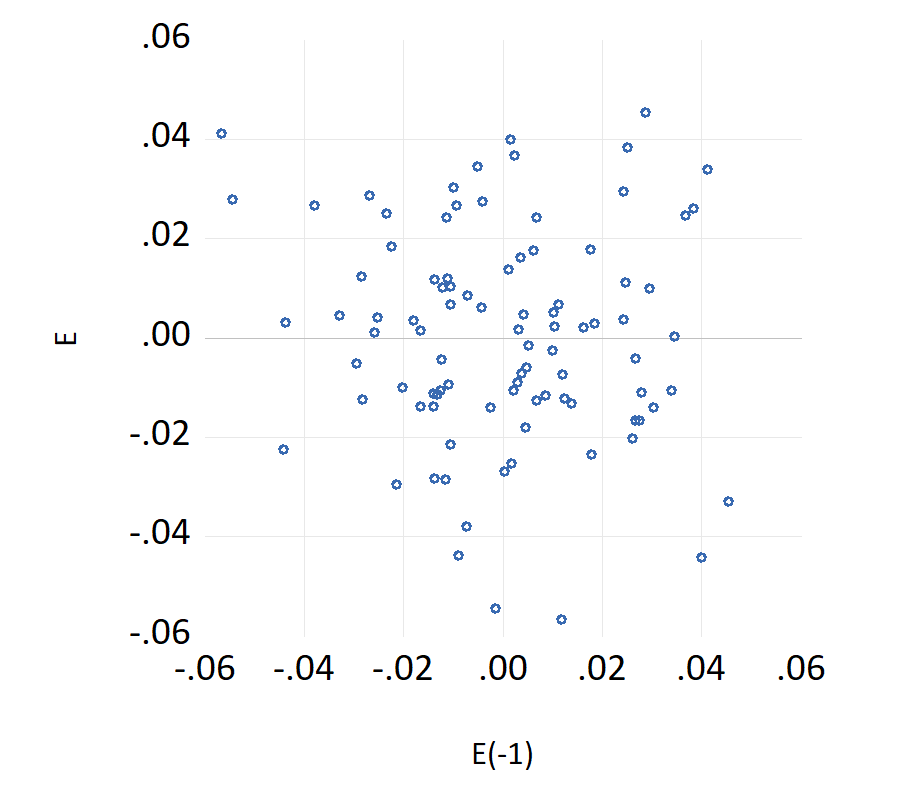
\includegraphics[width=0.75\textwidth]{./img/e-e(-1).png}
    \captionsetup{labelformat=empty}
    \caption{\textbf{\fontsize{9pt}{11pt}\selectfont 图5-8 残差自相关散点图}}
\end{figure}

从图5-7可以看出,残差序列图中残差呈现一定的规律性波动,初步判断可能存在自相关现象。图5-8中的残差自相关散点图进一步支持了这一判断。

为了更精确地验证自相关性问题,我们采用了Breusch-Godfrey LM检验,检验结果如表5.5所示。

\begin{table}[h!]
    \centering
    \captionsetup{labelformat=empty}
    \caption{\textbf{\fontsize{9pt}{11pt}\selectfont 表5.5 Breusch-Godfrey LM检验结果}}
    \begin{tabular}{lcc}
        \toprule
        检验统计量   & 统计量大小    & Prob.  \\
        \midrule
        F统计量    & 2.259496 & 0.0874 \\
        Obs*R平方 & 7.019040 & 0.0713 \\
        \bottomrule
    \end{tabular}
\end{table}

从表5.5中可以看出,p值大于0.05但是小于0.1,表明在10\%显著性水平下,模型存在自相关性问题。

\subsubsection{自相关问题的修正策略}
为了修正自相关性问题,我们采用了ARMA广义最小二乘法(GLS)进行回归分析,结果如表5.6所示。

\begin{table}[h!]
    \centering
    \captionsetup{labelformat=empty}
    \caption{\textbf{\fontsize{9pt}{11pt}\selectfont 表5.6 GLS回归结果}}
    \begin{tabular}{lccccc}
        \toprule
        变量       & 系数        & 标准误      & t值        & Prob.  \\
        \midrule
        常数项 (C)  & 0.230238  & 0.452410 & 0.508915  & 0.6121 \\
        CPI      & -0.001689 & 0.004535 & -0.372479 & 0.7105 \\
        INTEREST & -0.009547 & 0.011983 & -0.796731 & 0.4279 \\
        LOAN     & -3.86E-07 & 2.36E-07 & -1.638224 & 0.1051 \\
        M2       & 1.16E-08  & 1.53E-08 & 0.756582  & 0.4514 \\
        MC\_SH   & -4.14E-08 & 9.74E-08 & -0.425384 & 0.6716 \\
        R\_SZ    & 1.105133  & 0.050282 & 21.97347  & 0.0000 \\
        AR(1)    & -0.087798 & 0.114026 & -0.769981 & 0.4435 \\
        AR(2)    & -0.179594 & 0.110841 & -1.620280 & 0.1089 \\
        AR(3)    & 0.175483  & 0.109826 & 1.597825  & 0.1138 \\
        \bottomrule
    \end{tabular}
\end{table}

修正后的回归结果显示,自相关系数不再显著。为了验证自相关问题是否得到解决,我们再次采用Breusch-Godfrey LM检验,结果如表5.7所示。

\begin{table}[h!]
    \centering
    \captionsetup{labelformat=empty}
    \caption{\textbf{\fontsize{9pt}{11pt}\selectfont 表5.7 修正后Breusch-Godfrey LM检验结果}}
    \begin{tabular}{lcc}
        \toprule
        检验统计量   & 统计量大小    & Prob.    \\
        \midrule
        F统计量    & 0.753165 & 0.659401 \\
        Obs*R平方 & 1.499800 & 0.6821   \\
        \bottomrule
    \end{tabular}
\end{table}

从表5.7可以看出,p值远大于0.1,表明在10\%显著性水平下,修正后的模型中不存在自相关性问题,自相关问题得到了有效解决。



\subsection{多重共线性检验与修正}
\subsubsection{相关系数矩阵的构建}
基于构建的模型,我们计算了各个解释变量之间的相关系数,并得出相关系数矩阵如表5.8所示。

\begin{table}[h!]
    \centering
    \captionsetup{labelformat=empty}
    \caption{\textbf{\fontsize{9pt}{11pt}\selectfont 表5.8 相关系数矩阵}}
    \begin{tabular}{lcccccc}
        \toprule
                 & CPI       & INTEREST  & LOAN      & M2        & MC\_SH    & R\_SZ     \\
        \midrule
        CPI      & 1.000000  & -0.036364 & 0.031859  & -0.104015 & -0.064446 & -0.065456 \\
        INTEREST & -0.036364 & 1.000000  & 0.017355  & 0.254056  & -0.080723 & 0.088227  \\
        LOAN     & 0.031859  & 0.017355  & 1.000000  & 0.218616  & 0.164182  & -0.157384 \\
        M2       & -0.104015 & 0.254056  & 0.218616  & 1.000000  & 0.884414  & 0.012435  \\
        MC\_SH   & -0.064446 & -0.080723 & 0.164182  & 0.884414  & 1.000000  & 0.030587  \\
        R\_SZ    & -0.065456 & 0.088227  & -0.157384 & 0.012435  & 0.030587  & 1.000000  \\
        \bottomrule
    \end{tabular}
\end{table}

为了进一步判断模型中是否存在多重共线性,我们计算了相关系数矩阵的行列式。经Eviews计算得结果为0.096058,接近于零,初步判断模型中存在多重共线性问题。

\subsubsection{多重共线性问题的诊断与修正}
为了确定多重共线性的存在范围及表现形式,我们计算了各变量的方差膨胀因子(VIF),结果如下表5.9所示。

\begin{table}[h!]
    \centering
    \captionsetup{labelformat=empty}
    \caption{\textbf{\fontsize{9pt}{11pt}\selectfont 表5.9 方差膨胀因子(VIF)}}
    \begin{tabular}{lcccc}
        \toprule
        变量       & 系数方差     & 未中心化VIF  & 中心化VIF   \\
        \midrule
        C        & 0.223917 & 41236.41 & -        \\
        CPI      & 2.19E-05 & 40411.61 & 1.024994 \\
        INTEREST & 0.000181 & 1518.684 & 2.045561 \\
        LOAN     & 5.72E-14 & 3.664788 & 1.095220 \\
        M2       & 2.83E-16 & 230.7184 & 9.575526 \\
        MC\_SH   & 1.15E-14 & 274.7991 & 8.793140 \\
        R\_SZ    & 0.002501 & 1.054901 & 1.054782 \\
        \bottomrule
    \end{tabular}
\end{table}

从表5.11中可以看出,M2和MC\_SH的中心化VIF值接近10,说明这两个变量之间可能存在多重共线性问题。

为了修正多重共线性问题,我们逐步剔除了多重共线性严重的变量,并重新估计模型。首先剔除M2和MC\_SH变量,回归结果如表5.10所示。

\begin{table}[h!]
    \centering
    \captionsetup{labelformat=empty}
    \caption{\textbf{\fontsize{9pt}{11pt}\selectfont 表5.10 剔除M2和MC\_SH后的回归结果}}
    \begin{tabular}{lcccc}
        \toprule
        变量       & 系数        & 标准误      & t值        & Prob.  \\
        \midrule
        C        & 0.188240  & 0.468556 & 0.401745  & 0.6888 \\
        CPI      & -0.001640 & 0.004616 & -0.355304 & 0.7232 \\
        INTEREST & -0.002640 & 0.009420 & -0.280307 & 0.7799 \\
        LOAN     & -4.12E-07 & 2.31E-07 & -1.783792 & 0.0779 \\
        R\_SZ    & 1.100883  & 0.049415 & 22.27815  & 0.0000 \\
        \bottomrule
    \end{tabular}
\end{table}

最终,我们仅保留LOAN和R\_SZ变量进行回归分析,结果如表5.11所示。

\begin{table}[h!]
    \centering
    \captionsetup{labelformat=empty}
    \caption{\textbf{\fontsize{9pt}{11pt}\selectfont 表5.11 仅保留LOAN和R\_SZ变量的回归结果}}
    \begin{tabular}{lcccc}
        \toprule
        变量    & 系数        & 标准误      & t值        & Prob.  \\
        \midrule
        C     & 0.006231  & 0.004239 & 1.470024  & 0.1450 \\
        LOAN  & -4.15E-07 & 2.28E-07 & -1.819950 & 0.0721 \\
        R\_SZ & 1.100680  & 0.048633 & 22.63215  & 0.0000 \\
        \bottomrule
    \end{tabular}
\end{table}

通过逐步剔除多重共线性严重的变量,模型的VIF值显著降低,多重共线性问题得到了有效修正。修正后的方差膨胀因子(VIF)结果如表5.12所示。经过多重共线性修正后的模型如公式5-2所示。

\begin{equation}
    R\_SZ380 = 0.006231 + -4.15\times 10 ^ {-7} \times LOAN + 1.100680 \times R\_SZ
    \tag{5-2}
\end{equation}

\begin{table}[h!]
    \centering
    \captionsetup{labelformat=empty}
    \caption{\textbf{\fontsize{9pt}{11pt}\selectfont 表5.12 修正后方差膨胀因子(VIF)}}
    \begin{tabular}{lcccc}
        \toprule
        变量    & 系数方差     & 未中心化VIF  & 中心化VIF   \\
        \midrule
        C     & 1.80E-05 & 3.400628 & -        \\
        R\_SZ & 0.002365 & 1.025514 & 1.025399 \\
        LOAN  & 5.21E-14 & 3.431153 & 1.025399 \\
        \bottomrule
    \end{tabular}
\end{table}


\subsection{月度因素的引入与分析}
\subsubsection{虚拟变量的设置与估计}

基于经多重共线性修正的模型,为了进一步分析月度因素对上证380指数收益率的影响,我们以12月为基准月,采用加法方式引入了11个月度虚拟变量(MON1至MON11)。模型的回归结果如表5.13所示。

\begin{table}[h!]
    \centering
    \captionsetup{labelformat=empty}
    \caption{\textbf{\fontsize{9pt}{11pt}\selectfont 表5.13 引入月度虚拟变量后的回归结果}}
    \begin{tabular}{lcccc}
        \toprule
        变量    & 系数        & 标准误      & t值        & Prob.  \\
        \midrule
        C     & 0.002067  & 0.008723 & 0.236985  & 0.8133 \\
        R\_SZ & 1.073895  & 0.048044 & 22.35214  & 0.0000 \\
        LOAN  & -3.52E-07 & 2.89E-07 & -1.220691 & 0.2258 \\
        MON1  & -0.010302 & 0.012829 & -0.802987 & 0.4244 \\
        MON2  & 0.020075  & 0.011152 & 1.800166  & 0.0756 \\
        MON3  & 0.017662  & 0.011609 & 1.521409  & 0.1321 \\
        MON4  & -0.009929 & 0.011150 & -0.890435 & 0.3759 \\
        MON5  & 0.001183  & 0.011159 & 0.106055  & 0.9158 \\
        MON6  & 0.012753  & 0.011481 & 1.110781  & 0.2700 \\
        MON7  & 0.008285  & 0.011163 & 0.742207  & 0.4601 \\
        MON8  & 0.017707  & 0.011142 & 0.153189  & 0.8786 \\
        MON9  & -0.000511 & 0.011297 & -0.045268 & 0.9640 \\
        MON10 & -0.001785 & 0.011204 & -0.159282 & 0.8738 \\
        MON11 & -0.002253 & 0.011553 & -0.195027 & 0.8459 \\
        \bottomrule
    \end{tabular}
\end{table}

\subsubsection{月度因素影响的分析}

从表5.13的回归结果可以看出,月度虚拟变量对上证380指数收益率的影响并不显著。在11个月度虚拟变量中,仅有2月份(MON2)在10\%的显著性水平下显著,系数为0.020075,说明2月份对上证380指数收益率有一定的正向影响。这可能与春节前后市场活跃度增加有关。然而,其他月份的虚拟变量均未表现出显著性,表明月度因素对上证380指数收益率的整体影响较弱。

综合来看,月度虚拟变量的引入并未显著提升模型的解释力,但揭示了2月份对上证380指数收益率的特定影响。未来的研究可以进一步探讨其他时间因素对股市收益率的影响,或结合更多的市场事件进行分析,以期得到更为深入的结论。

\subsection{变量的平稳性与协整关系检验}
\subsubsection{变量的平稳性检验}
为了保证模型的有效性和准确性以完成协整关系检验,我们首先对所有变量进行平稳性检验。平稳性检验是确保变量不存在单位根的重要步骤,通常采用增强型Dickey-Fuller(ADF)检验来判断时间序列的平稳性。表5.14是各变量的平稳性检验结果。

\begin{table}[h!]
    \centering
    \captionsetup{labelformat=empty}
    \caption{\textbf{\fontsize{9pt}{11pt}\selectfont 表5.14 各变量的ADF检验结果}}
    \begin{tabular}{lcc}
        \toprule
        变量       & t值        & Prob.  \\
        \midrule
        CPI      & -7.951497 & 0.0000 \\
        INTEREST & -2.551976 & 0.1068 \\
        LOAN     & -11.07517 & 0.0000 \\
        M2       & 2.435444  & 1.0000 \\
        MC\_SH   & -1.400595 & 0.5788 \\
        R\_SZ    & -11.18157 & 0.0000 \\
        R\_SZ380 & -10.77701 & 0.0000 \\
        \bottomrule
    \end{tabular}
\end{table}

从表5.14的检验结果可以看出,CPI、LOAN、R\_SZ和R\_SZ380变量在1\%显著性水平下是平稳的,而INSERT、M2、MC\_SH不平稳,是趋势序列。对于不平稳的变量,我们需要对其进行差分处理以达到平稳性。我们可以进一步对平稳变量进行协整检验。

\subsubsection{协整关系与格兰杰因果检验}

为了分析被解释变量 R\_SZ380 与解释变量 R\_SZ、LOAN、DCPI 之间的长期均衡关系,我们首先进行协整检验。其中,DCPI 为 CPI 一阶差分后的平稳序列,用于协整检验和误差修正模型分析。根据 Johansen 协整检验方法,我们得到了表5.15结果。结果表明,R\_SZ380 与 R\_SZ、LOAN、DCPI 之间存在协整关系。这意味着尽管短期内可能存在偏离,但是这些变量之间存在长期均衡关系。

\begin{table}[h!]
    \centering
    \captionsetup{labelformat=empty}
    \caption{\textbf{\fontsize{9pt}{11pt}\selectfont 表5.15 协整检验结果}}
    \begin{tabular}{lcccc}
        \toprule
        假设的协整关系数量            & 特征值      & 迹统计量     & 临界值 (0.05) & Prob.  \\
        \midrule
        无协整关系 (None)         & 0.406480 & 117.8360 & 47.85613   & 0.0000 \\
        最多一个协整关系 (At most 1) & 0.285824 & 70.36275 & 29.79707   & 0.0000 \\
        最多两个协整关系 (At most 2) & 0.221311 & 39.72980 & 15.49471   & 0.0000 \\
        最多三个协整关系 (At most 3) & 0.170098 & 16.96673 & 3.841465   & 0.0000 \\
        \bottomrule
    \end{tabular}
\end{table}

为了进一步分析变量之间的因果关系,我们进行了格兰杰因果检验,结果如表 5.16 所示。进一步的格兰杰因果检验结果表明,R\_SZ、LOAN 和 CPI 与 R\_SZ380 之间并不存在明显的格兰杰因果关系。这表明大多数变量之间在短期内没有显著的格兰杰因果关系,只有LOAN对CPI的变化具有显著的预测能力。

\begin{table}[h!]
    \centering
    \captionsetup{labelformat=empty}
    \caption{\textbf{\fontsize{9pt}{11pt}\selectfont 表5.16 格兰杰因果检验结果}}
    \begin{tabular}{lcc}
        \toprule
        假设                       & F统计量    & Prob.  \\
        \midrule
        R\_SZ 不是 R\_SZ380 的格兰杰因果 & 1.24026 & 0.3003 \\
        R\_SZ380 不是 R\_SZ 的格兰杰因果 & 1.00477 & 0.3949 \\
        LOAN 不是 R\_SZ380 的格兰杰因果  & 0.86914 & 0.4605 \\
        R\_SZ380 不是 LOAN 的格兰杰因果  & 0.35619 & 0.7848 \\
        CPI 不是 R\_SZ380 的格兰杰因果   & 1.84466 & 0.1453 \\
        R\_SZ380 不是 CPI 的格兰杰因果   & 2.16625 & 0.0980 \\
        LOAN 不是 R\_SZ 的格兰杰因果     & 0.42367 & 0.7365 \\
        R\_SZ 不是 LOAN 的格兰杰因果     & 0.09427 & 0.9630 \\
        CPI 不是 R\_SZ 的格兰杰因果      & 1.50409 & 0.2194 \\
        R\_SZ 不是 CPI 的格兰杰因果      & 1.64294 & 0.1856 \\
        CPI 不是 LOAN 的格兰杰因果       & 0.60506 & 0.6135 \\
        LOAN 不是 CPI 的格兰杰因果       & 4.05526 & 0.0096 \\
        \bottomrule
    \end{tabular}
\end{table}
\subsubsection{误差修正模型的估计与分析}

在确定了 R\_SZ380 与 R\_SZ、LOAN、DCPI 之间存在协整关系后,我们进一步估计误差修正模型,结果如表 5.17 所示。结果显示,误差修正项的系数为负且显著,表明存在误差修正机制。此外,D(R\_SZ)、D(LOAN) 和 D(DCPI) 对 D(R\_SZ380) 具有显著的影响,分别表现为市场规模、贷款和物价指数的变动对股票市场收益的显著影响。

\begin{table}[h!]
    \centering
    \captionsetup{labelformat=empty}
    \caption{\textbf{\fontsize{9pt}{11pt}\selectfont 表5.17 误差修正模型结果}}
    \begin{tabular}{lcc}
        \toprule
        变量        & t值        & Prob.  \\
        \midrule
        C         & -0.041027 & 0.9674 \\
        D(R\_SZ)  & 26.93276  & 0.0000 \\
        D(LOAN)   & -4.257540 & 0.0001 \\
        D(DCPI)   & -3.545206 & 0.0006 \\
        E\_T6(-1) & -10.19873 & 0.0000 \\
        \bottomrule
    \end{tabular}
\end{table}

\subsection{VAR模型的估计与脉冲响应分析}
\subsubsection{VAR模型的构建与最优滞后项确定}

为了分析上证指数收益率(R\_SZ)、人民币新增贷款增长率(D(lnLOAN))、沪市A股总市值增长率(D(lnMC\_SH))之间的动态关系,我们构建了三元VAR模型。根据表5.18的信息准则法(AIC,SC,HQ),我们确定VAR模型的最优滞后阶数为2。

\begin{table}[h!]
    \centering
    \captionsetup{labelformat=empty}
    \caption{\textbf{\fontsize{9pt}{11pt}\selectfont 表5.18 VAR滞后阶数选择}}
    \begin{tabular}{lcccccc}
        \toprule
        滞后阶数 & LogL     & LR       & FPE      & AIC       & SC        & HQ        \\
        \midrule
        0    & 239.5884 & NA       & 7.67e-07 & -5.566785 & -5.480574 & -5.532108 \\
        1    & 292.1654 & 100.2057 & 2.75e-07 & -6.592127 & -6.247283 & -6.453421 \\
        2    & 314.6692 & 41.30112 & 2.01e-07 & -6.909864 & -6.306386 & -6.667128 \\
        3    & 322.1889 & 13.27001 & 2.08e-07 & -6.875033 & -6.012291 & -6.528267 \\
        4    & 325.5672 & 5.723223 & 2.38e-07 & -6.742758 & -5.622012 & -6.291962 \\
        5    & 329.1828 & 5.870994 & 2.72e-07 & -6.616067 & -5.236687 & -6.061242 \\
        6    & 339.4861 & 16.00032 & 2.67e-07 & -6.646731 & -5.008718 & -5.987876 \\
        7    & 343.0835 & 5.332613 & 3.07e-07 & -6.519611 & -4.622964 & -5.756727 \\
        8    & 352.9047 & 13.86530 & 3.06e-07 & -6.538935 & -4.383654 & -5.672020 \\
        \bottomrule
    \end{tabular}
\end{table}

在确定了最优滞后阶数2后,我们对VAR模型进行了估计。VAR模型的估计结果(表5.19)显示,上证指数收益率(R\_SZ)的变化与人民币新增贷款增长率(D(lnLOAN))和沪市A股总市值增长率(D(lnMC\_SH))之间存在复杂的动态关系。从结果来看,R\_SZ的自身滞后项对其未来的变化有显著影响,这表明历史的上证指数收益率对未来收益率具有一定的预测能力。

此外,联合系数检验结果(表5.20)表明,虽然个别变量的滞后项对其他变量的影响不显著,但整体来看,VAR模型能够较好地捕捉到变量之间的相互影响。例如,D(lnMC\_SH)的变化对R\_SZ有显著影响,这表明沪市A股总市值增长率是影响上证指数收益率的重要因素之一。而D(lnLOAN)对R\_SZ的影响则相对较弱。

综上所述,VAR模型在最优滞后阶数为2的情况下,能够有效地捕捉上证指数收益率、人民币新增贷款增长率和沪市A股总市值增长率之间的动态关系。通过对模型的估计和联合系数检验,我们可以更好地理解这些经济变量之间的相互作用,为未来的经济预测和政策制定提供科学依据。

\begin{table}[h!]
    \centering
    \captionsetup{labelformat=empty}
    \caption{\textbf{\fontsize{9pt}{11pt}\selectfont 表5.19 VAR模型估计结果}}
    \begin{tabular}{lcccc}
        \toprule
        变量              & R\_SZ      & D(lnLOAN)  & D(lnMC\_SH) \\
        \midrule
        R\_SZ(-1)       & 0.019499   & 3.250449   & 0.653221    \\
                        & (0.16757)  & (2.23967)  & (0.11326)   \\
                        & [1.45131]  & [5.76763]  & [2.15720]   \\
        R\_SZ(-2)       & 0.010261   & -0.089866  & 0.268716    \\
                        & (0.18431)  & (2.46333)  & (0.12457)   \\
                        & [0.55668]  & [-0.03648] & [2.15720]   \\
        D(lnLOAN(-1))   & -0.000333  & -0.906021  & -1.75e-05   \\
                        & (0.04816)  & (0.09515)  & (0.00481)   \\
                        & [-9.52230] & [-0.00364] & [-0.00364]  \\
        D(lnLOAN(-2))   & -0.002774  & -0.467859  & -0.002053   \\
                        & (0.03824)  & (0.09297)  & (0.00340)   \\
                        & [-5.03254] & [-0.43678] & [-0.43678]  \\
        D(lnMC\_SH(-1)) & -0.139027  & -4.478695  & -0.506441   \\
                        & (0.24874)  & (3.32447)  & (0.16811)   \\
                        & [-1.34719] & [-3.01250] & [-3.01250]  \\
        D(lnMC\_SH(-2)) & -0.053706  & 3.644561   & -0.117968   \\
                        & (0.30491)  & (2.35416)  & (0.11905)   \\
                        & [-1.54814] & [-0.99095] & [-0.99095]  \\
        C               & 0.001991   & 0.001567   & 0.007380    \\
                        & (0.00465)  & (0.06215)  & (0.00314)   \\
                        & [0.42830]  & [0.02521]  & [2.34841]   \\
        \bottomrule
    \end{tabular}
\end{table}

\begin{table}[h!]
    \centering
    \captionsetup{labelformat=empty}
    \caption{\textbf{\fontsize{9pt}{11pt}\selectfont 表5.20 VAR模型联合系数检验结果}}
    \begin{tabular}{lccc}
        \toprule
        被解释变量       & 排除变量        & $\chi^2$ 统计量 & Prob.  \\
        \midrule
        R\_SZ       & D(lnLOAN)   & 0.304373     & 0.8588 \\
                    & D(lnMC\_SH) & 0.350593     & 0.8392 \\
                    & 全部          & 0.732843     & 0.9472 \\
        D(lnLOAN)   & R\_SZ       & 2.801856     & 0.2464 \\
                    & D(lnMC\_SH) & 5.277043     & 0.0715 \\
                    & 全部          & 5.376063     & 0.2508 \\
        D(lnMC\_SH) & R\_SZ       & 33.74356     & 0.0000 \\
                    & D(lnLOAN)   & 0.311216     & 0.8559 \\
                    & 全部          & 34.67906     & 0.0000 \\
        \bottomrule
    \end{tabular}
\end{table}



\subsubsection{脉冲响应函数的估计与解读}

为了分析上证指数收益率(R\_SZ)、人民币新增贷款增长率(D(lnLOAN))、沪市A股总市值增长率(D(lnMC\_SH))之间的动态关系,我们对构建的VAR模型进行了脉冲响应函数分析。图5-9展示了各变量对自身和其他变量的冲击响应。从脉冲响应函数的估计结果可以看出,R\_SZ 对自身冲击具有较强的短期效应,但在中长期内逐渐消失。而对 D(lnLOAN) 和 D(lnMC\_SH) 的冲击响应较为微弱,表明人民币新增贷款增长率和沪市A股总市值增长率对上证指数收益率的影响较小。D(lnLOAN) 和 D(lnMC\_SH) 对自身冲击也具有显著的短期效应,但相互之间的影响不显著。

因此,通过脉冲响应函数分析,我们发现上证指数收益率在短期内受自身因素的影响较大,而人民币新增贷款增长率和沪市A股总市值增长率对其影响较小。

\begin{figure}[h!]
    \centering
    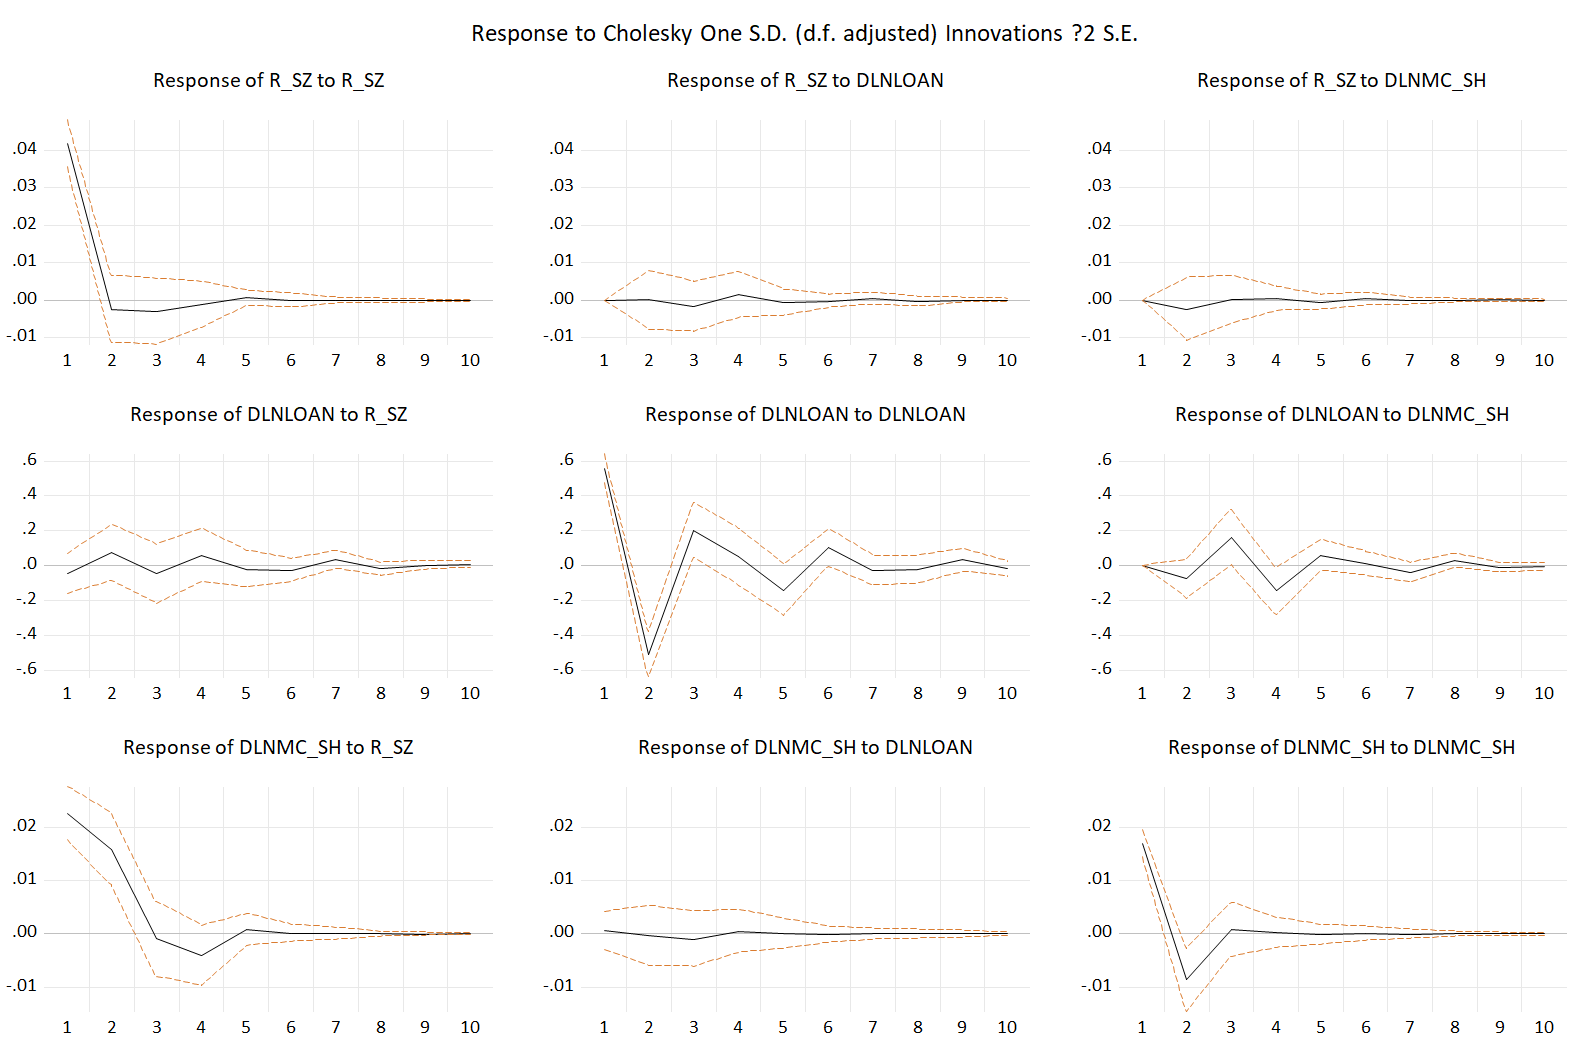
\includegraphics[width=\textwidth]{./img/impulse.png}
    \captionsetup{labelformat=empty}
    \caption{\textbf{\fontsize{9pt}{11pt}\selectfont 图5-9 脉冲响应函数估计结果}}
\end{figure}

\subsection{GARCH模型的估计与波动性分析}
\subsubsection{均值方程的构建}

基于2016-01-01至2024-01-01上证指数(000001)的日收益率(R\_SZ)数据,首先进行描述性统计分析,如表5.21所示。可以看出,R\_SZ的均值接近于零,中位数略高于均值,表明收益率的分布稍有右偏。同时,R\_SZ的最大值和最小值分别为0.0571和-0.0772,显示出较大的波动性。标准差为0.0109,进一步证明了收益率的高波动性。

\begin{table}[h!]
    \centering
    \captionsetup{labelformat=empty}
    \caption{\textbf{\fontsize{9pt}{11pt}\selectfont 表5.21 R\_SZ的描述性统计}}
    \begin{tabular}{lc}
        \toprule
        指标  & R\_SZ     \\
        \midrule
        均值  & -2.93E-05 \\
        中位数 & 0.000300  \\
        最大值 & 0.057100  \\
        最小值 & -0.077200 \\
        标准差 & 0.010917  \\
        偏度  & -0.859411 \\
        峰度  & 9.615543  \\
        \bottomrule
    \end{tabular}
\end{table}

接着,进行变量的平稳性检验,如表5.22所示,结果表明R\_SZ在1\%、5\%、10\%的显著性水平下拒绝原假设,因此R\_SZ为平稳序列。

\begin{table}[h!]
    \centering
    \captionsetup{labelformat=empty}
    \caption{\textbf{\fontsize{9pt}{11pt}\selectfont 表5.22 R\_SZ的ADF单位根检验结果}}
    \begin{tabular}{lccccc}
        \toprule
        变量    & t统计量      & 临界值(1\%)  & 临界值(5\%)  & 临界值(10\%) & Prob.  \\
        \midrule
        R\_SZ & -46.00905 & -3.433514 & -2.862824 & -2.567500 & 0.0000 \\
        \bottomrule
    \end{tabular}
\end{table}

随后,初步估计AR模型的阶数。通过比较AIC和BIC信息准则(图5-10),初步选择AR(5)模型,如表5.23所示。AR(5)模型较为显著,且通过进一步检验发现AR(4)(表5.24)模型效果不如AR(5)。此外,AR(6)模型虽然同样显著,但增加了模型复杂度。因此,最终选择AR(5)模型作为均值方程的形式进行后续的GARCH模型估计与波动性分析。

\begin{figure}[h!]
    \centering
    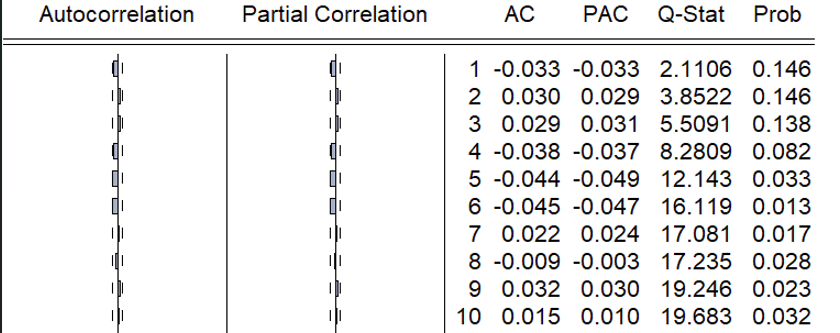
\includegraphics[width=0.8\textwidth]{./img/ar.png}
    \captionsetup{labelformat=empty}
    \caption{\textbf{\fontsize{9pt}{11pt}\selectfont 图5-10 信息准则}}
\end{figure}

\begin{table}[h!]
    \centering
    \captionsetup{labelformat=empty}
    \caption{\textbf{\fontsize{9pt}{11pt}\selectfont 表5.23 AR(5)模型估计结果}}
    \begin{tabular}{lcccc}
        \toprule
        变量    & 系数        & 标准误      & t统计量      & Prob.  \\
        \midrule
        AR(1) & -0.022508 & 0.022697 & -0.991660 & 0.3215 \\
        AR(2) & 0.037193  & 0.022463 & 1.655729  & 0.0979 \\
        AR(3) & 0.011085  & 0.022444 & 0.493892  & 0.6214 \\
        AR(4) & -0.035026 & 0.022436 & -1.561109 & 0.1187 \\
        AR(5) & -0.047994 & 0.022215 & -2.160418 & 0.0309 \\
        \bottomrule
    \end{tabular}
\end{table}

\begin{table}[h!]
    \centering
    \captionsetup{labelformat=empty}
    \caption{\textbf{\fontsize{9pt}{11pt}\selectfont 表5.24 AR(4)模型估计结果}}
    \begin{tabular}{lcccc}
        \toprule
        变量    & 系数        & 标准误      & t统计量      & Prob.  \\
        \midrule
        C     & 3.01E-05  & 0.000238 & 0.126093  & 0.8997 \\
        AR(1) & -0.025143 & 0.022478 & -1.118554 & 0.2635 \\
        AR(2) & 0.037174  & 0.022459 & 1.655158  & 0.0981 \\
        AR(3) & 0.009442  & 0.022465 & 0.420280  & 0.6743 \\
        AR(4) & -0.037804 & 0.022231 & -1.700560 & 0.0892 \\
        \bottomrule
    \end{tabular}
\end{table}

\subsubsection{残差的序列自相关}

为了检验均值方程残差项的序列自相关性,采用了图示法和解析法。图示法通过观察残差的自相关函数(ACF)和偏自相关函数(PACF)图,以及残差平方项的自相关函数和偏自相关函数图,解析法通过ARCH效应检验进行检验。

首先,观察均值方程残差的ACF和PACF图(如图5-11所示)。从图中可以看出,残差的自相关函数和偏自相关函数在大部分滞后期内并没有显著偏离零,表明残差项不存在显著的序列自相关性。

\begin{figure}[h!]
    \centering
    \captionsetup{labelformat=simple}
    \begin{minipage}[b]{0.45\textwidth}
        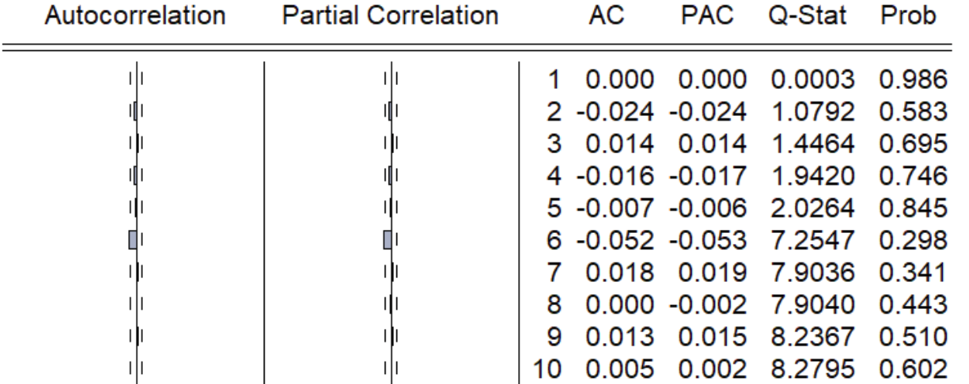
\includegraphics[width=\textwidth]{./img/r.png}
        \captionsetup{labelformat=empty}
        \caption{\textbf{\fontsize{9pt}{11pt}\selectfont 图5-11 残差的ACF和PACF}}
    \end{minipage}
    \hfill
    \begin{minipage}[b]{0.45\textwidth}
        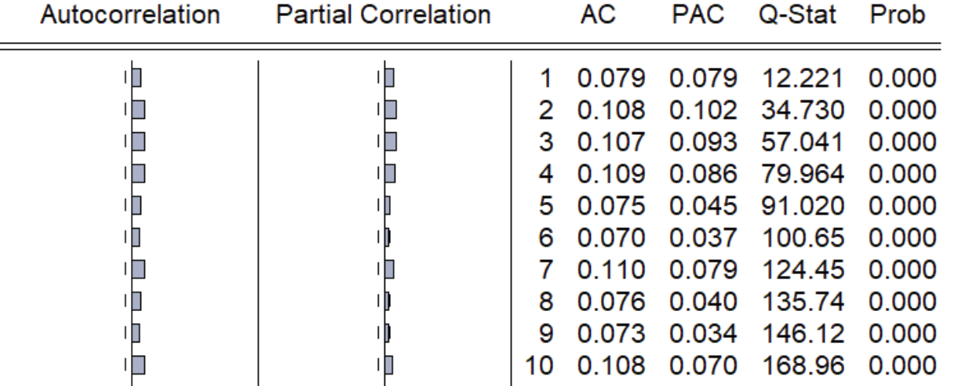
\includegraphics[width=\textwidth]{./img/r2.png}
        \captionsetup{labelformat=empty}
        \caption{\textbf{\fontsize{9pt}{11pt}\selectfont 图5-12 残差平方项的ACF和PACF}}
    \end{minipage}
    \captionsetup{labelformat=empty}
\end{figure}


其次,观察均值方程残差平方项的ACF和PACF图(如图5-12所示)。从图中可以看出,残差平方项的自相关函数和偏自相关函数在部分滞后期内显著偏离零,表明残差平方项存在显著的序列自相关性。

最后,通过ARCH效应检验对残差平方项进行解析检验,结果如表5.25所示。可以看出,ARCH检验的F统计量和Obs*R-squared统计量的p值均小于0.05,拒绝无序列自相关的原假设,进一步表明残差平方项存在显著的序列自相关性。

\begin{table}[h!]
    \centering
    \captionsetup{labelformat=empty}
    \caption{\textbf{\fontsize{9pt}{11pt}\selectfont 表5.25 ARCH效应检验}}
    \begin{tabular}{lcccc}
        \toprule
        变量            & 系数       & 标准误      & t统计量     & Prob.  \\
        \midrule
        RESID$^2$(-1) & 0.054466 & 0.022696 & 2.399789 & 0.0165 \\
        RESID$^2$(-2) & 0.078292 & 0.022647 & 3.457096 & 0.0006 \\
        RESID$^2$(-3) & 0.086089 & 0.022634 & 3.803518 & 0.0001 \\
        RESID$^2$(-4) & 0.070957 & 0.022628 & 3.135852 & 0.0017 \\
        RESID$^2$(-5) & 0.046138 & 0.022227 & 2.075760 & 0.0380 \\
        \bottomrule
    \end{tabular}
\end{table}

综上所述,均值方程的残差项不存在显著的序列自相关性,而残差平方项存在显著的序列自相关性,说明存在ARCH效应。通过对均值方程残差的序列自相关性分析,验证了进一步进行GARCH模型估计的必要性。

\subsubsection{GARCH模型构建与波动性分析}

基于前面的分析结果,我们构建了GARCH(1,1)和GARCH(2,1)模型,并对模型进行估计。结果如表5.26和表5.27所示。

\begin{table}[h!]
    \centering
    \captionsetup{labelformat=empty}
    \caption{\textbf{\fontsize{9pt}{11pt}\selectfont 表5.26 GARCH(1,1)模型估计结果}}
    \begin{tabular}{lcccc}
        \toprule
        变量            & 系数        & 标准误      & z统计量      & Prob.  \\
        \midrule
        AR(1)         & 0.005799  & 0.024269 & 0.238946  & 0.8111 \\
        AR(2)         & 0.003843  & 0.024922 & 0.154210  & 0.8774 \\
        AR(3)         & 0.021620  & 0.025057 & 0.862823  & 0.3882 \\
        AR(4)         & -0.040836 & 0.024307 & -1.679981 & 0.0930 \\
        AR(5)         & -0.057675 & 0.022833 & -2.525916 & 0.0115 \\
        C             & 1.93E-06  & 3.37E-07 & 5.716961  & 0.0000 \\
        $RESID(-1)^2$ & 0.078213  & 0.005707 & 13.70518  & 0.0000 \\
        GARCH(-1)     & 0.905199  & 0.006337 & 142.8332  & 0.0000 \\
        \bottomrule
    \end{tabular}
\end{table}

\begin{table}[h!]
    \centering
    \captionsetup{labelformat=empty}
    \caption{\textbf{\fontsize{9pt}{11pt}\selectfont 表5.27 GARCH(2,1)模型估计结果}}
    \begin{tabular}{lcccc}
        \toprule
        变量            & 系数        & 标准误      & z统计量      & Prob.  \\
        \midrule
        AR(1)         & -0.006370 & 0.027813 & -0.229042 & 0.8188 \\
        AR(2)         & 0.003216  & 0.023998 & 0.134025  & 0.8934 \\
        AR(3)         & 0.023108  & 0.023366 & 0.988988  & 0.3227 \\
        AR(4)         & -0.041232 & 0.022666 & -1.819101 & 0.0689 \\
        AR(5)         & -0.059311 & 0.021572 & -2.749385 & 0.0060 \\
        C             & 1.28E-06  & 2.55E-07 & 5.011816  & 0.0000 \\
        $RESID(-1)^2$ & 0.158410  & 0.014115 & 11.22262  & 0.0000 \\
        $RESID(-2)^2$ & -0.102293 & 0.016109 & -6.350095 & 0.0000 \\
        GARCH(-1)     & 0.932226  & 0.007409 & 125.8267  & 0.0000 \\
        \bottomrule
    \end{tabular}
\end{table}

根据估计结果,GARCH(1,1)和GARCH(2,1)模型的均值方程和条件方差方程分别为公式5-3与公式5-4所示。

\begin{equation}
    \left\{
    \begin{aligned}
        R_{SZ} & = 0.005799 \, AR(1) + 0.003843 \, AR(2) + 0.021620 \, AR(3)                \\
               & \quad - 0.040836 \, AR(4) - 0.057675 \, AR(5)                              \\
        h_t    & = 1.93 \times 10^{-6} + 0.078213 \, \epsilon_{t-1}^2 + 0.905199 \, h_{t-1}
    \end{aligned}
    \right. \tag{5-3}
\end{equation}

\begin{equation}
    \left\{
    \begin{aligned}
        R_{SZ} & = -0.006370 \, AR(1) + 0.003216 \, AR(2) + 0.023108 \, AR(3)                                              \\
               & \quad - 0.041232 \, AR(4) - 0.059311 \, AR(5)                                                             \\
        h_t    & = 1.28 \times 10^{-6} + 0.158410 \, \epsilon_{t-1}^2 - 0.102293 \, \epsilon_{t-2}^2 + 0.932226 \, h_{t-1}
    \end{aligned}
    \right. \tag{5-4}
\end{equation}

通过对比两个模型的结果,可以看出GARCH(2,1)模型在拟合效果上优于GARCH(1,1)模型,因此选择GARCH(2,1)模型作为最终的分析模型。GARCH(2,1)模型的条件方差方程中,滞后期数为1和2的残差平方项均显著,这表明波动性具有较强的自相关性。


\newpage
\section{结果与讨论}
\subsection{分析、启示与局限性}
在本研究中,我们综合运用了多元线性回归和GARCH模型对上证380指数收益率的影响因素及其波动性进行了全面分析。分析结果揭示了上证指数收益率(R\_SZ)和金融机构新增贷款金额(LOAN)对上证380指数收益率(R\_SZ380)具有显著影响,其中上证指数收益率对(R\_SZ380)有正向作用,而金融机构新增贷款金额则呈现负向影响,突显了市场趋势和信贷政策在影响指数收益中的重要性。

其次,通过一系列的统计检验与修正,包括对数变换、一阶差分和广义最小二乘法,我们确保了回归结果的稳健性,消除了初始模型的异方差、自相关、多重共线性等问题。此外,GARCH模型的波动性分析,特别是GARCH(2,1)模型,为我们提供了对收益率波动自相关性和动态模式的深层理解。

对于市场参与者,我们的研究提供了一些启示。如,投资者应密切关注市场整体表现,并考虑信贷政策对市场流动性和资金供给的潜在负面影响。此外,特定月份的季节性市场活动增加,如2月份的春节,可能对收益率产生正向影响,这为投资者提供了时间上的投资策略参考。同时,GARCH模型揭示的波动性特征对风险管理和资产配置具有指导意义。

然而,本文的研究有局限性。模型选择和构建方面,多元线性回归模型会在捕捉非线性关系和高频数据波动性方面存在不足。未来的研究可以通过引入非线性或机器学习模型来提高预测精度。数据的频率和样本范围也是未来研究可以改进的方向,使用更高频率的数据,如分钟级数据,将有助于更精确地捕捉市场波动。

并且,虽然在实证分析中采用统计方法修正模型有助于解决问题,但也可能引入新的偏误。因此,我们在解释模型结果时,应结合经济学理论和市场实际情况,保持谨慎态度。

综上所述,本文的研究不仅识别了影响上证380指数收益率的关键因素,也揭示了其波动性特征,为投资者和政策制定者提供了一定参考。未来的研究应当在模型构建和数据应用上进行更深层次的探索和创新,以期获得更加全面和深入的理解。

\subsection{未来研究方向}
在认识到本文研究局限性的同时,我们认为未来的研究可以从如下几个方面着手。

首先,我们可以探索更复杂的非线性或机器学习模型,以增强对市场动态的捕捉能力。这些模型将有助于提高我们对市场现象预测的精度和深度。

其次,我们可以采用更高频率的数据,并结合宏观经济变量和市场情绪指标,以全面分析其对指数收益率的影响。通过数据扩展,研究者可以更精细地捕捉市场的高频波动特征。

此外,我们还可以将研究范围扩展至其他股票市场,如美股、港股等。跨市场的分析将有助于我们更全面地理解不同市场的运行机制和特点。

最后,我们可以结合重大经济事件或政策变化,进行事件研究,分析这些事件对指数收益率的短期和长期影响。

综上所述,通过这些改进,未来的研究将有助于揭示上证380指数收益率的更深层次动态特性,为投资者和政策制定者提供更加全面和深入的见解。

\newpage
\begin{center}
    {\heiti \fontsize{18pt}{18pt}\selectfont 参考文献}
\end{center}
\vspace{12pt}

\begin{enumerate}[label={[}\arabic*{]}]
    \item 于雪皎. 上证指数收益率波动研究[J]. 经济管理杂志, 2013.
    \item 顾鹏. 宏观冲击与股票收益率———基于日度数据的分析[J]. 财经问题研究, 2014, 10(371): 66-71.
    \item 杨科, 林洪. 中国股市波动率与收益率的因果关系研究[J]. 统计与决策, 2010(21).
    \item 李腊生, 翟淑萍, 关敏芳. 证券市场收益率分布时变性的经济学分析及其我国的经验证据[J]. 统计研究, 2011, 28(11).
    \item 王元月, 梁翠翠. 基于变参数模型的流动性与上证综指收益率关系研究[J]. 中国管理科学, 2010, 18(2).
    \item 陈守东, 陈雷, 刘艳武. 中国沪深股市收益率及波动性相关分析[J]. 金融研究, 2003(7).
    \item 王晓芳, 王瑞君. 上证综指波动特征及收益率影响因素研究——基于EEMD和VAR模型分析[J]. 南开经济研究, 2012, 6.
\end{enumerate}

% Appendix
\newpage
\begin{center}
    {\heiti\zihao{2} 附录}
\end{center}
\zihao{4}

由于篇幅限制,文章中没有给出数据下载的过程以及Eviews的原始图表。由于文章改为线下提交,这部分内容会单独提交到学习通原文章线上提交处。
\end{document}
